\chapter{Hacheur 4 quadrants}

Le schéma général du dispositif est celui de la figure suivante:

\begin{figure}[h]
\centering

\includegraphics[width=\linewidth]{TP_H4Q/fig/TP_H4Q.png}
%\caption{Simplified internal control}
\end{figure}

L’alimentation $U_E$ est réalisée par un redressement triphasé du réseau 50 Hz variable jusqu'à 400 V au moyen d'un autotransformateur, suivi d’un condensateur de filtrage de valeur $C$. La machine à courant continu est à excitation indépendante qui sera maintenue constante avec un courant d'excitation égal à sa valeur nominale.

L’ensemble ``redresseur-hacheur'' est réalisé au sein d’un dispositif intégré SEMIKRON muni d’un système de commande externe permettant de réaliser une commande complémentaire synchrone ou décalée sur chacun des deux ``bras de pont''.

Le dispositif de commande permet de générer des signaux PWM dont le rapport cyclique peut être commandé à l'aide d'un potentiomètre ou une tension externe $v(t)$ \textbf{entre 0 et 5V}.

\newpage
\section{Préparation}

On commande le hacheur avec les signaux de commande $f_1$, $f_2$, $f_3$ et $f_4$ ci-dessous. 

\begin{enumerate}
\item Tracer l'évolution de la tension de sortie du hacheur $U_m(t)$ en supposant que la tension d'entrée $U_e(t)$ est parfaitement constante.
\item Calculer la valeur moyenne de $U_m(t)$ en fonction de la tension d'entrée $U_e$ (supposée constante) et $\alpha$.
\end{enumerate}

\begin{figure}[h]
\centering
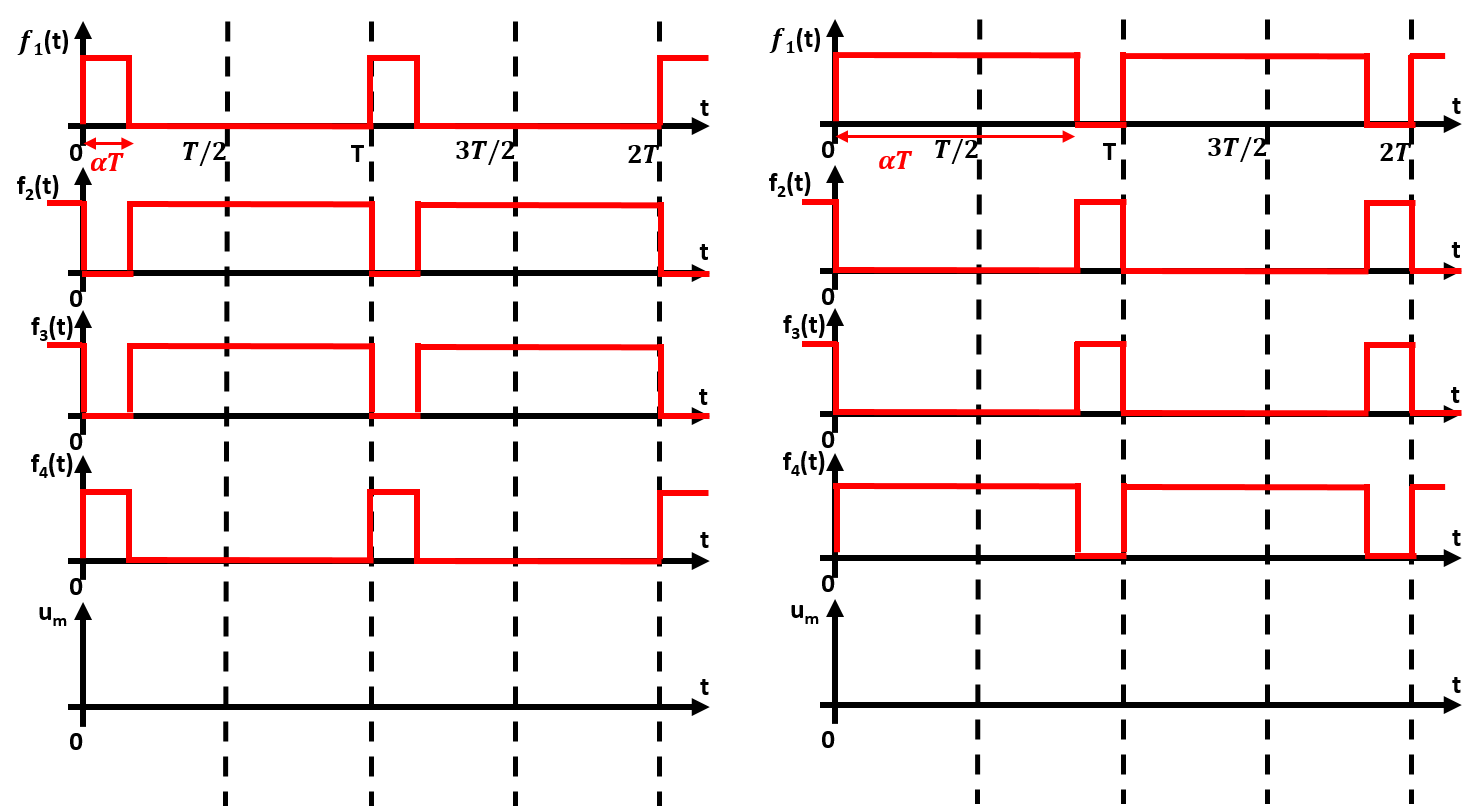
\includegraphics[width=1.1\linewidth]{TP_H4Q/fig/prepa_synchrone.png}
%\caption{Simplified internal control}
\end{figure}


\newpage
\section{Réalisation du montage}

\begin{enumerate}
\item Relever les caractéristiques de la machine à courant continu et en déduire la valeur de la tension continue redressée $U_E$ nécessaire pour pouvoir exploiter toute la plage de vitesse de cette machine dans les deux sens. On majorera cette valeur ``théorique'' de $U_E$ de 20 \% pour tenir compte des chutes de tension et des limitations de rapport cycliques inhérentes à la boîte de commande.

\item Relever l’allure des signaux de commande notés $COM$ et $\overline{COM}$ sur la boîte de commande. (on n'utilisera pas les signaux $DEC$ et $\overline{DEC}$) \textbf{On s'assurera que le rapport cyclique soit différent de 50 \%}. En déduire:
\begin{itemize}
\item Le branchement des signaux de contrôle $COM$ et $\overline{COM}$
\item L’allure de la tension de sortie du hacheur, notamment son amplitude et sa fréquence.
\end{itemize}

\item Tracer la caractéristique de réglage de cette commande, i.e. le rapport cyclique de la commande $COM$ en fonction de la tension de commande externe (\textbf{variable dans l’intervalle 0 à 5V}). En déduire la valeur de cette tension imposant l’arrêt de la machine.

\item Réaliser le montage complet avec les recommandations suivantes:
\begin{itemize}
\item laisser la machine à courant continu à vide;
\item si la machine est à excitation séparée, câbler en premier lieu son excitation et vérifier la valeur du courant correspondant;
\item régler la commande du hacheur pour imposer un rapport cyclique de 50\%;
\item augmenter progressivement la tension réseau (autotransformateur) jusqu’à atteindre la tension redressée $U_E$ souhaitée;
\item tester le bon fonctionnement du dispositif en faisant varier la commande du hacheur \textbf{lentement} dans les deux sens et en surveillant en permanence l’intensité du courant d’induit moteur.
\end{itemize}

Le montage étant assez ``volumineux'' à réaliser, il faudra prendre soin de câbler les différents blocs entre eux de manière aisément vérifiable. Les différents appareils de mesure devront être lisibles et l’oscilloscope sera aussi éloigné que possible des connexions de puissance.

\item Si le freinage du moteur est trop rapide, la tension de bus continu $U_E$ augmente. Pourquoi ? \underline{\textbf{En présence de l'enseignant}}, observer ce phénomène.
\end{enumerate}

\section{Caractérisation ``statique'' du dispositif}

\begin{enumerate}[label={}]
\item \textbf{En vérifiant toujours que $U_E$ reste constante}, tracer la caractéristique du hacheur $<U_m>=f(\alpha)$, le moteur étant laissé à vide ($\alpha$ représente le rapport cyclique de la commande $COM$). Relever soigneusement les valeurs extrêmes de rapport cycliques possibles, $\alpha_{min}$ et $\alpha_{max}$.

\end{enumerate}

\section{Etude du hacheur en régime dynamique}

Dans cette étude, il faut générer un rapport cyclique du type : $\alpha(t) = \alpha_0 + \Delta\alpha(t)$ où $\Delta\alpha(t)$ est une variation ``lente'' et $\alpha_0 = 0.5$. Pour cela, la tension de commande utilisée pour piloter le dispositif comprend une composante continue $v_0$ et une composante alternative de fréquence faible, notée $\Delta v(t)$. On laissera toujours le moteur à vide \textbf{et l’on prendra soin de ne pas commuter les fonctions du générateur de commande avec un montage sous tension} afin d’éviter les surintensités.

\begin{enumerate}
\item Utiliser la caractéristique de réglage précédente pour déterminer $v_0$ et $\Delta v(t)$ afin de faire varier le rapport cyclique linéairement entre 0.25 et 0.75. Appliquer cette tension progressivement sur le dispositif (amplitude lentement augmentée), à une fréquence de cycle de 0.3 Hz environ (fréquence du signal $\Delta v$).

\item Relever alors simultanément le courant d’induit moteur $i_M$ et la tension mesurée par la génératrice tachymétrique $v_T$ (image de la vitesse $\Omega$). Comment interpréter ces courbes en utilisant le mode XY de l’oscilloscope (avec une rémanence suffisante) ? On pourra améliorer la mesure en intercalant un filtre passe bas sur la mesure du courant afin d’éliminer son ondulation. Comment choisir la fréquence de coupure de ce filtre ?

\item Observer simultanément la vitesse, le courant d'induit et la tension d'entrée $U_e(t)$. Expliquer les variations observées sur $U_e(t)$ et lier celles-ci aux 4 quadrants de fonctionnement.

\end{enumerate}

\section{Onduleur}

Remplacer le moteur par une charge R - L série. On souhaite alimenter cette charge avec le réseau électrique nord-américain (110V / 60 Hz) à partir de notre réseau (230V / 50 Hz). On va donc utiliser le hacheur en ``onduleur'' monophasé afin de récréer ce réseau. Pour cela, on utilisera un rapport cyclique de la forme $\alpha(t) = \alpha_0 + \delta\alpha. sin(\omega t)$
\begin{enumerate}
\item Déterminer $\alpha_0$, $\delta\alpha$ et $\omega$ afin de recréer le réseau désiré.

\item Appliquer cette commande et alimenter la charge. Observer la tension $U_m$ en sortie du hacheur et $U_r$ la tension aux bornes de la résistance.

\end{enumerate}



